\chapter{Introduzione al progetto}

\section{Descrizione dell'applicazione}



\section{Primi requisiti funzionali}
Di seguito sono riportati i primi requisiti funzionali ricavati dal processo di analisi delle richieste del committente, ottenute durante le interviste iniziali del progetto. Tali requisiti definiscono le funzionalità e i servizi 
offerti dal sistema da realizzare.

\begin{center}
       \captionof{table}{Primi requisiti funzionali}

    \begin{tabular}{p{6cm}|p{8cm}}

    \toprule
    \multicolumn{1}{c}{\textbf{Requisito funzionale}} &
    \textbf{Descrizione}\\

    \midrule
    Login ai servizi & Permettere all'utente l'accesso ai servizi bancari mediante credenziali \\\\
    Visualizzazione riepilogo conti e carte & Fornire opportune viste di riepilogo dei prodotti posseduti da un utente (esempio: conti correnti, carte di credito, ecc\dots)\\\\
    Visualizzazione storico saldi & Rappresentare tramite grafici dello storico saldi di un prodotto\\\\
    Riepilogo lista movimenti & Recuperare e visualizzare la lista dei movimenti di un determinato prodotto\\\\
    Filtraggio lista movimenti & Permettere il recupero dei movimenti in base un certo arco temporale\\\\
    Disporre operazioni bancarie & Permettere l'esecuzione di dispositive bancarie (esempio: bonifici, giroconti, ecc\dots) \\\\
    Interazione con i social network & Consentire la visualizzazione dei contenuti social messi a disposizione del cliente\\\\
    Messaggistica & Permettere la lettura delle comunicazioni ricevute  \\\\
    \bottomrule

    \end{tabular}
        \label{tab:requisiti_iniziali}

\end{center}



\section{Primi mockup, wireframe e prototipi}
\subsection{Mockup}
La realizzazione di mockup grafici ha permesso di offrire al cliente una prima rappresentazione visiva dei requisiti funzionali iniziali. Di seguito sono riportate alcuni di questi mockup relativi allo stadio iniziale del progetto.

\begin{figure}[!htbp]
\centering
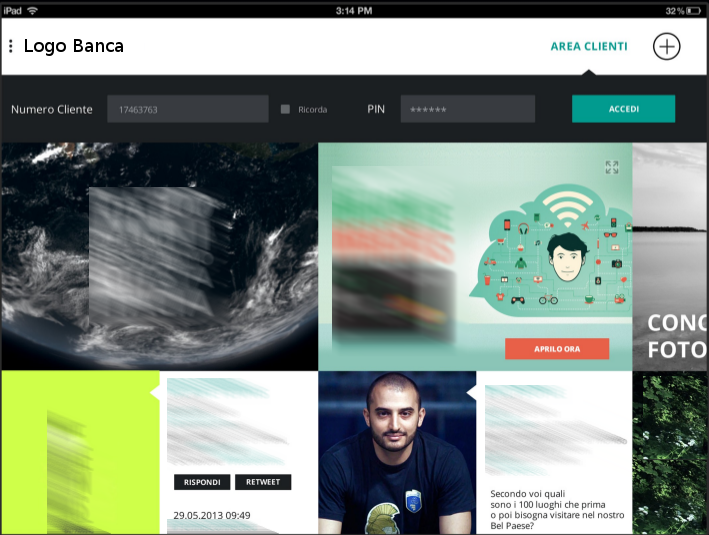
\includegraphics[scale=0.7]{immagini_mockup/home.png}
\caption{Home contenuti social e pannello login}
\end{figure}

\begin{figure}[!htbp]
\centering
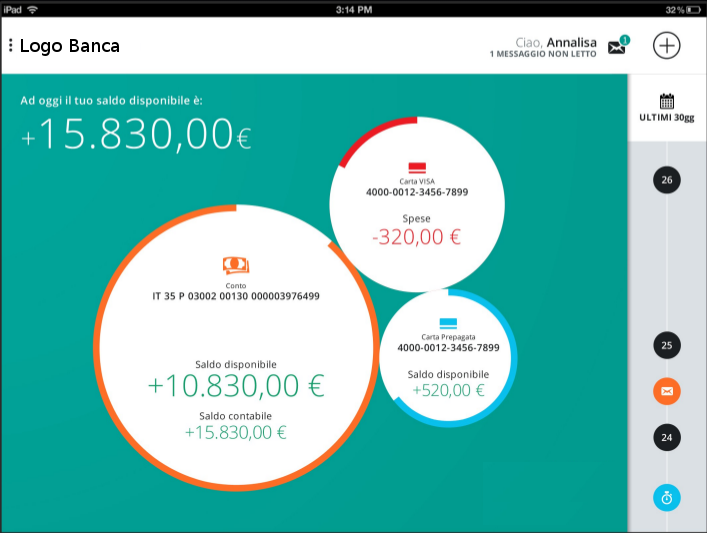
\includegraphics[scale=0.7]{immagini_mockup/bolle.png}
\caption{Riepilogo conti e carte}
\end{figure}

\begin{figure}[!htbp]
\centering
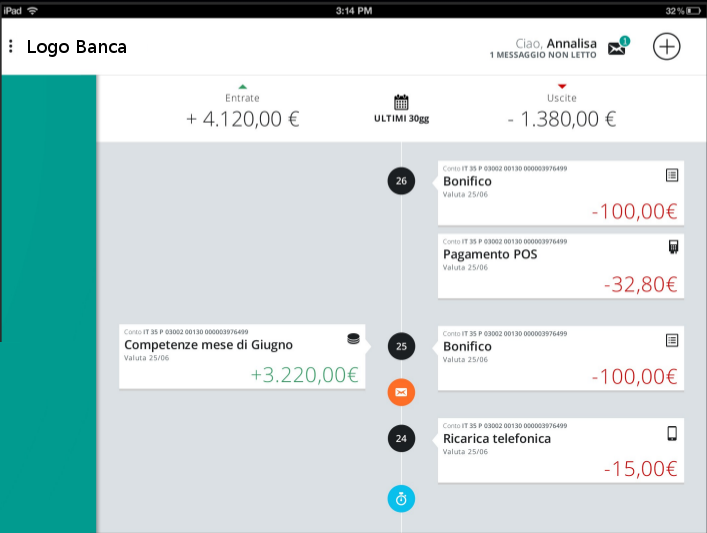
\includegraphics[scale=0.7]{immagini_mockup/timeline.png}
\caption{Timeline movimenti}
\end{figure}

\begin{figure}[!h]
\centering
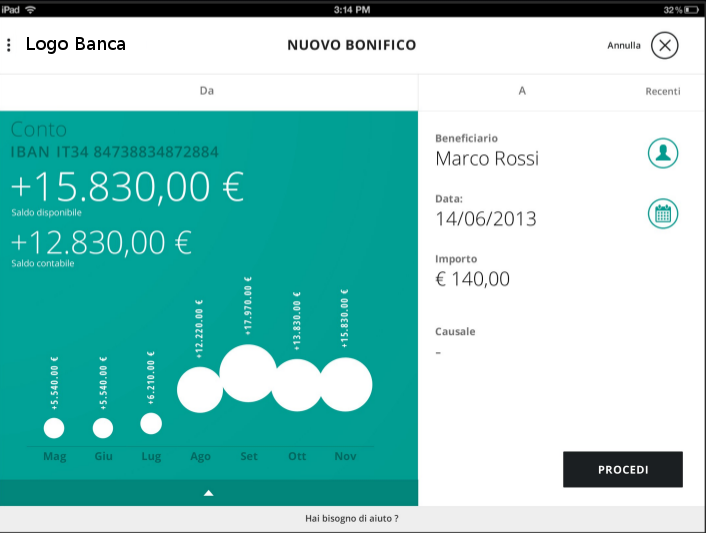
\includegraphics[scale=0.7]{immagini_mockup/bonifico.png}
\caption{Operazione bonifico}
\end{figure}

\newpage
\subsection{Wireframe}
Parallelamente ai mockup e durante tutto il ciclo di vita del software sono stati realizzati e raffinati i wireframe. 

I wareframe forniscono una rappresentazione strutturale di un applicazione software e permettono di individuare le dinamiche del progetto in termini di usabilità ed utilizzo pratico, i punti critici e quelli che richiedono uno sviluppo più accurato o miglioramenti.

Di seguito sono mostrate alcune delle immagini di uno dei primi wireframe realizzati:

\begin{figure}[!htbp]
\centering
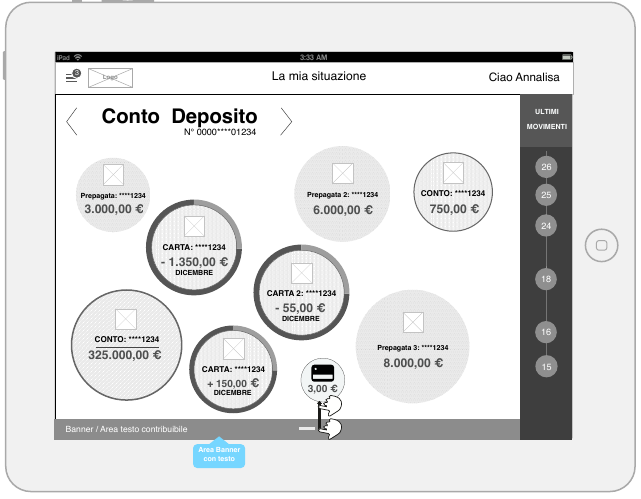
\includegraphics[scale=1.0]{primo_wireframe/miasituazione.png}
\caption{Riepilogo conti e carte}
\end{figure}
\begin{figure}[!htpb]
\centering
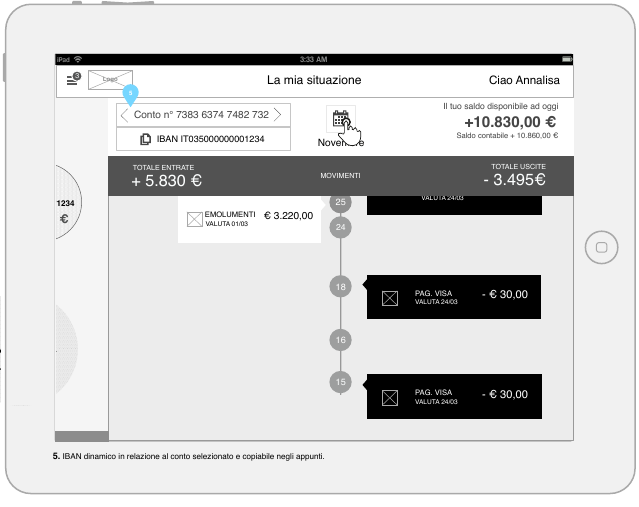
\includegraphics[scale=1.0]{primo_wireframe/timeline2.png}
\caption{Timeline movimenti}
\end{figure}
\begin{figure}[!htbp]
\centering
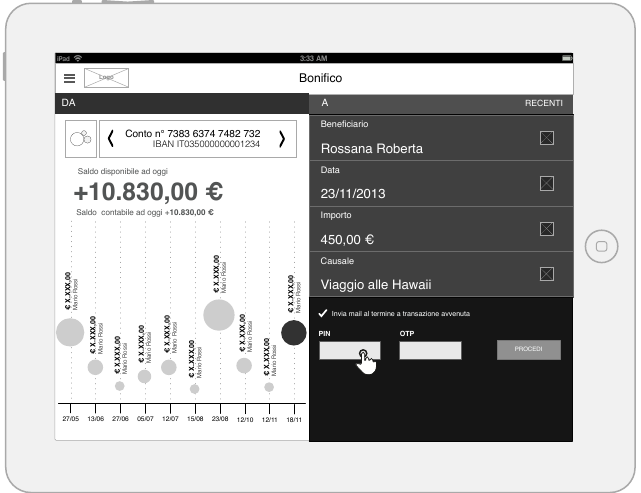
\includegraphics[scale=1.0]{primo_wireframe/bonifico2.png}
\caption{Dettaglio bonifico}
\end{figure}

\newpage
\subsection{Prototipi}
Un'altro passo fondamentale durante la fase iniziale del progetto è stato la realizzazione di prototipi.

Un prototipo è un modello approssimato del sistema che si sta realizzando e che simula o esegue solo una parte delle funzioni del sistema finale.
La prototipizzazione permette di:

\begin{itemize}
  \item tenere il design centrato sull’utente 
  \item sperimentare design alternativi
  \item ottenere feedback rapidi sul progetto
  \item trascurare dettagli secondari (come qualità del codice, efficienza, ecc\dots) 
  \item valutare l'usabilità
  \item ridurre i rischi di un progetto permettendoci di mettere prima a fuoco alcune caratteristiche del sistema e capire se sono adeguate o meno
\end{itemize}

Durante le prime settimane del progetto sono stati quindi realizzati dei prototipi contenenti funzionalità \emph{stub}\footnote{Funzionalità che simulano il comportamento  del sistema restituendo valori accettabili in un ipotetico scenario reale.} descritte dalla tabella \ref{tab:requisiti_iniziali}. Tali prototipi sono stati successivamente messi a disposizione del cliente e testati su device Apple iPad, portando alla raccolta e valutazione dei primi feedback sull'utilizzo del software.
